\subsection{Stability}
We associate a set of binary variables $s(f)(d)$ indicating the stability of $f$ at depth $d$. Here the depth can be interpolated as the following procedure. $Lf$, $Rf$, and all fold lines on the background patches are stable at depth 0. Now if we add two patches between background patches forming a stable structure, the corresponding fold line will be stable at depth 1. We can continue to add stable structure based on current structure and the depth increases as the procedure goes on.

We use the idea of forming the popup by iteratively adding stable structure to formulate the stability constraint. That is, we check a building block at depth $d$ to see whether it is stable or not based on previous building blocks (with stability depth less than $d$).


% Note that we only consider stability for active fold lines. A key additional variable $same\_patch(f_s, f_t)$ indicates whether $f_s$ and $f_t$ are on the same final patch. $same\_patch(f_s, f_t) = 1$ when $P(f_s, f_t)$ exists and its fold lines are all inactive (meaning the patch is not folded). (See figure \ref{fig:path}.) With $same\_patch(f_s, f_t)$, we can sum up with support from all fold lines on the same patch to form constraints as $\#(f_t) <= \sum_s{*(f_s)c(f_s, f_t)}$ (see figure \ref{fig:support} for details).

% \begin{figure}[h]
%   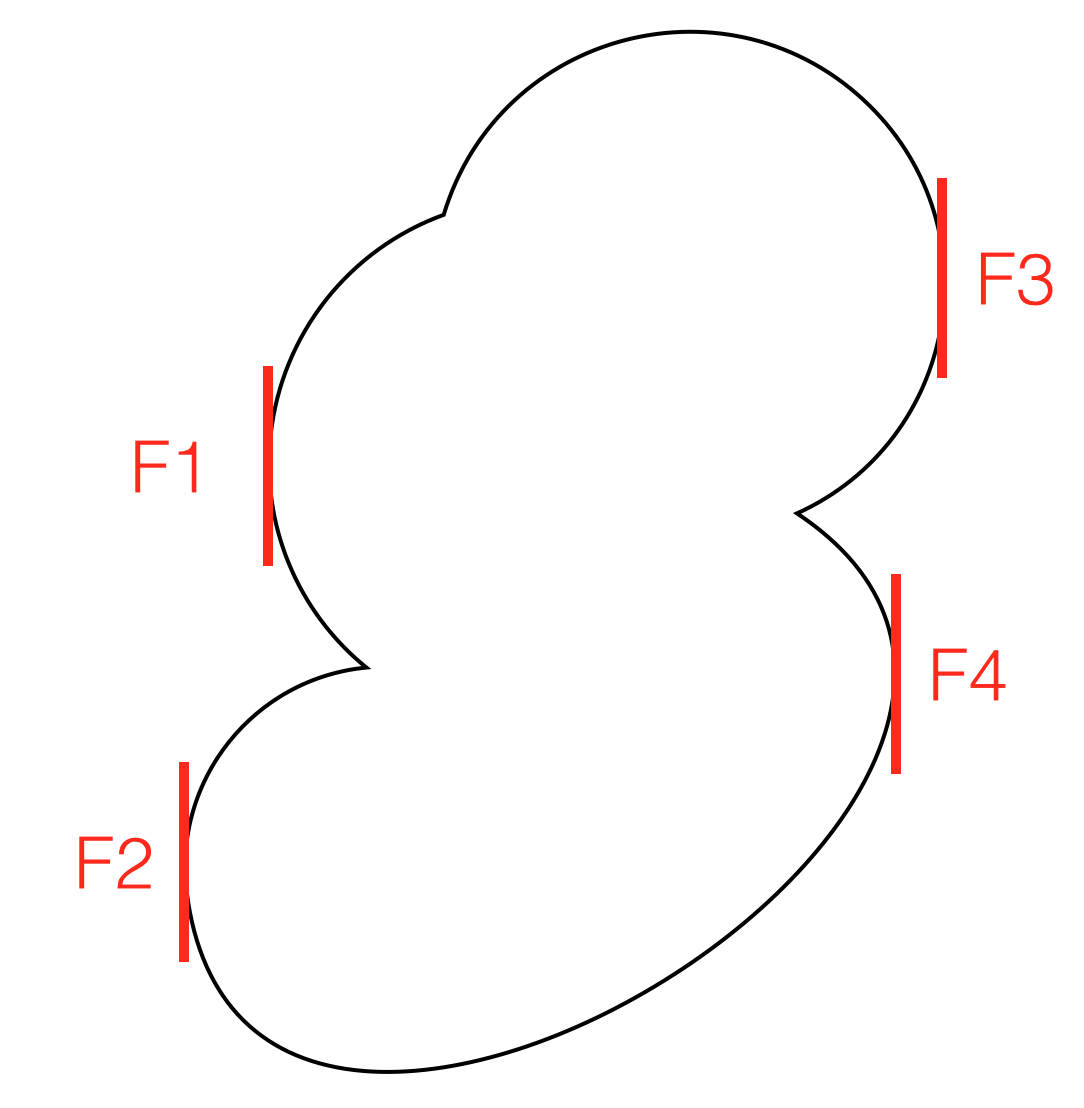
\includegraphics[width = 0.3\textwidth]{Figures/support}
%   \caption{Suppose these four fold lines are on the same final patch (determined by same\_patch($f_i$, $f_j$) = 1). Then the attribute for each fold line results from the support from all these four fold lines. To be more specific, for these four fold lines, we have the following. 1) If two or more fold lines are stable, then other fold lines are also stable. 2) If one fold line is stable, then other fold lines is called as ``directly connected'' which means a fold line is directly connected with a stable fold line (has only one degree of freedom). 3) If two or more fold lines are ``directly connected'', then other fold lines are called ``double-connected'' which means a fold line is not directly connected with stable fold lines but has two connection with stable fold lines. 4) If one fold line is ``double-connected'', then other fold lines is called as ``extended'' (used for certain cases).}
%   \label{fig:support}
% \end{figure}

% With the notation in figure \ref{fig:support}, a fold line is stable if one of the follows holds:

% \begin{enumerate}
% \item It is on the same patch with two stable fold lines.
% \item It is ``directly connected'' with a stable patch from the left and ``directly connected'' with a stable patch from the right.
% \item It is ``double-connected'' with a stable patch from the left and ``double-connected'' with a stable patch from the right.
% \item It is ``directly connected'' with a stable patch from the left and ``double-connected'' with a stable patch from the right (or vice versa).
% \item It is ``extended'' with a stable patch from the left and ``double-connected'' with a stable patch from the right (or vice versa).
% \end{enumerate}

We consider five types of stable structure:
\begin{enumerate}
\item A fold line is stable if it is on the same patch with two known stable fold lines. (\cite{li2010popup})
\item A fold line is stable if it is on the same patch with one known stable fold line and on another patch with another known stable fold line. (\cite{li2010popup})
\item A fold line is on a B-path or F-path. (\cite{le2014surface})
\item A fold line is double connected with two stable patches (ours).
\item A fold line is double connected with a stable patch and directly connect with a stable patch (or a patch which is double connected with a stable patch) (ours).
\end{enumerate}

    These cases are illustrated in figure \ref{fig:stable}.

\begin{figure}[h]
  
\includegraphics[width = 0.2\textwidth]{Figures/stable_1}
  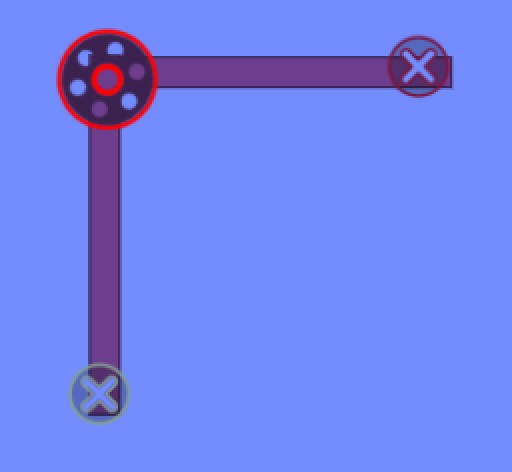
\includegraphics[width = 0.2\textwidth]{Figures/stable_2}
  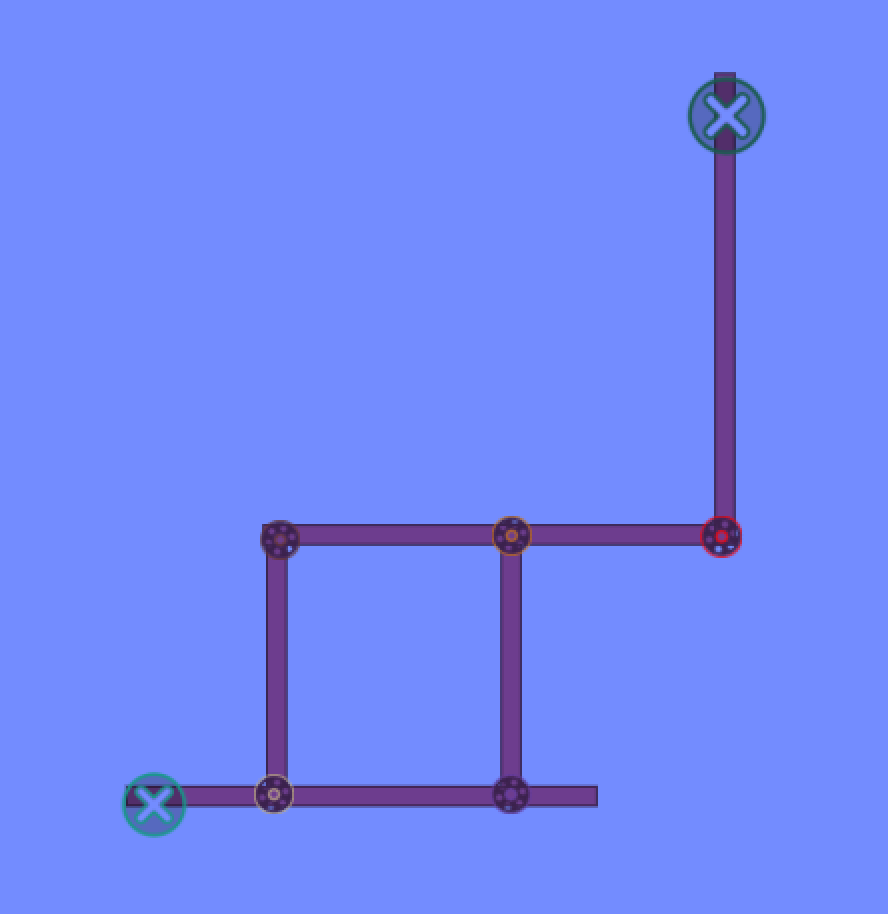
\includegraphics[width = 0.2\textwidth]{Figures/stable_3}
  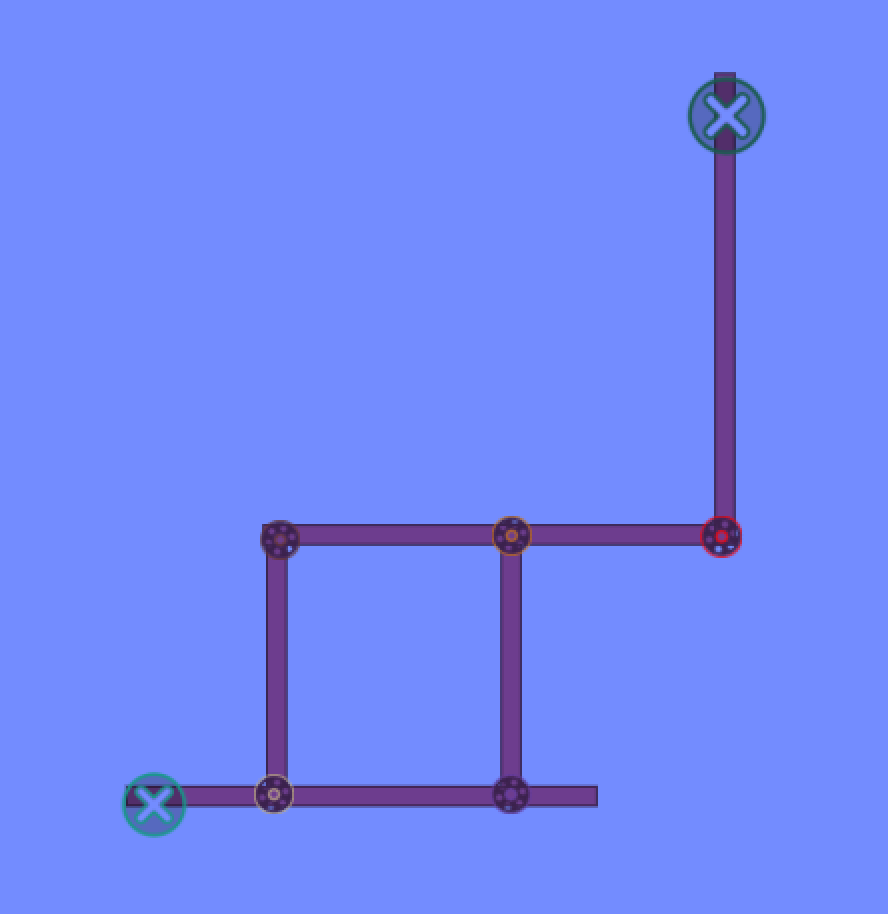
\includegraphics[width = 0.2\textwidth]{Figures/stable_4}
  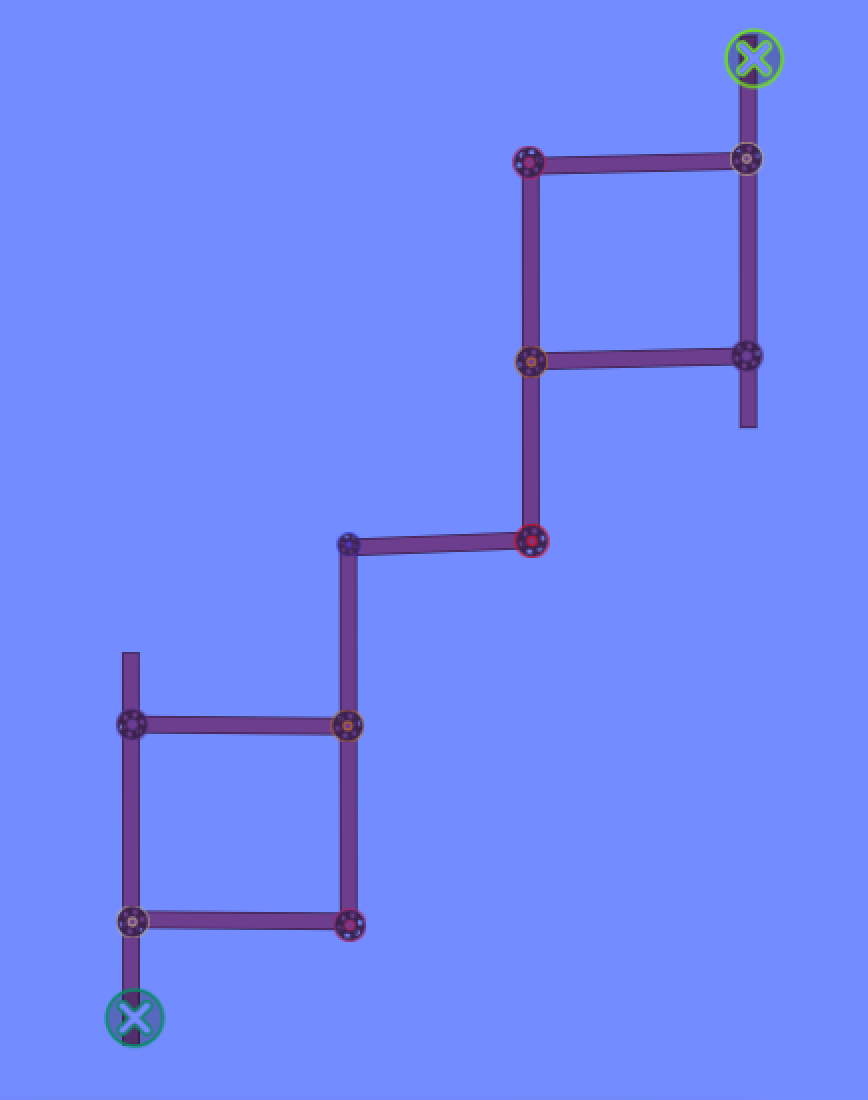
\includegraphics[width = 0.2\textwidth]{Figures/stable_5}
  \caption{The anchor with X sign represents a stable fold line and the anchor with red color is the fold line to be considered}
  \label{fig:stable}
\end{figure}

The process of determining stability is as follows:
\begin{enumerate}
\item Background fold lines are stable with stability depth 0.
\item For stability depth k, we find either the above structures based on the stable fold lines with stability depth less than k, and mark fold line in such structures as stable with stability k.
\item Repeat this process until all fold lines are marked as stable at some point. (We set a stability depth limit in practice.)
\end{enumerate}